The previous chapter addressed the validity of elimination of relaxed memory accesses. 
We also showed how validity of loop invariant code motion can be done using reordering coupled with elimination of events. 
In this concluding chapter, we discuss the limitations of our approach from a practical standpoint.
We later chart out further steps that can be taken from our work that we find important to address.
We then give our critique of the model in terms of mixed size and tear-free factor of accesses. 
We finally conclude with possible future work in the domain of relaxed memory models.
\ \newline
\ \newline  
\hrule 
\ \newline 
\ \newline 

\section{Limitations/Advantages}

    Throughout this thesis, we dealt with program transformations using abstract set of events and partial order relations. 
    Additionally, contrast to relying on operational semantics for our reasoning, we relied in a relatively simple and clear axiomatic semantics. 
    This approach however, is not without its limitations. 
    We elicit the key ones we think that are important. 

    \paragraph{Separation of Concerns}
    Our approach to program transformations avoids the algorithmic complexity of program transformations. 
    We do not assume why the compiler would perform such a transformation.
    While this benefits our analysis to be independent of any particular optimization, it may pose as a bottleneck while trying to incorporate our results in practice. 
    As a simple example, it might turn out to be that sequentially, a conditional will always return $true$ (the conditional variable may be local to the thread). 
    This would mean that no candidate execution can have events from the $false$ branch. 
    Hence the compiler might choose to reorder the events within the $true$ branch outside. 
    But as per Corollary \ref{ReordCond}, we do not allow any reordering outside the conditional, simply because we have no such information about the fact that a conditional always returns the same value. 
    Having such information can give us more fine grained analysis of when reordering is valid for different optimizations. 
    On the other hand, having such a separation can help compiler writers see the impact of the model on the basic program transformations clearly, thus allowing them to write relatively correct program transformation algorithms and even design new ones incorporating the impact of the model. 

    \paragraph{Validity of Transformations is a conservative}
    \critic{red}{Discuss with Clark what does it mean for our approach to be sound but not complete. Or is it that conservative analysis is not about soundness of completeness at all?}

    It is important to note that our approach to validity of elimination and reordering is conservative.
    We do not assume anything about events that belong to other agents/threads. 
    We only use information on the events involved in the program transformation and those that are \textit{agent-ordered} between them.
    There could be several cases where one could reorder or eliminate events that we prohibit, but are still safe to do. 
    From the perspective of the semantics of the memory model, this is possible because certain \textit{happens-before} relations may not be relevant; they do not "trigger" any of the axioms of the model, if removed. 
    Hence, such a transformation can be valid. 
    This, however, as mentioned before, is specific to certain programs. 
    To keep track of such information while doing program transformation in practice would be infeasible as the program size increases.
    
    \paragraph{Lack of Practical Results}
    This work is purely theoretical. 
    There is yet much more to be done to extend our results into practice. 
    The main reason we resorted to first a theoretical guarantee is because literature has shown that mere empirical testing of results on concurrent programs is insufficient. 
    Methods such as model checking, only work reasonably well for small programs. 
    While this is another approach to identify counter examples to program transformations, it is infeasible in practice due to the sheer magnitude of possible candidate executions.

    \paragraph{Mapping from Programming Constructs to Abstract events}
    The specification and the results on program transformations are purely at the abstract set of shared memory accesses.
    The concise mapping from ECMAScript's Read/Write(s) to these abstract events is something that must be done to extend our results in practice.
    As an example, we might have to perform aliasing analysis to identify which shared memory accesses are of same range. 
    Such mappings however, are not required for our results; they do not influence it in any way.
  
 

   

\section{Steps Further}

    We elicit in this section the complete road-map we had in mind during hte inception of this thesis. 
    We believe these are the following steps that anyone can take using our results to move towards practical relevance.

    \paragraph{Addressing Read-Modify-Write}
        So far we have assumed that no read modify write events exist in programs.
        However, this assumption is too strong in general (eg: Compare-and-Swap, Atomic Increment/Decrement are often used in programs).
        The validity of reordering/elimination when RMW events are involved should be done to have a complete analysis of these two transformations as far as shared memory accesses are concerned.

    \paragraph{Incorporating Tearing Factor}
        The role of tearing is still not clear to us.
        Axiom \ref{TfRe} does not rely on any partial order relations other than reads-from. 
        Since our approach is mainly reliant on preserving happens-before, our intuition is that our results should ideally be independent of the tearing factor.
        However, a proof including tearing events is still needed.   
  
    \paragraph{Role of synchronize/host-specific events}
        We have not yet considered the role of synchronize events. 
        Though for a programmer this is equivalent to wait and notify, reordering and elimination under their presence is something we have not conisdered. 
        This we suspect would require understanding the operational aspect of wait / notify procedures.

        We do not yet know how Host Specific synchronize events work with relaxed memory accesses.
        Strictly speaking, their semantics from a consistency model perspective is given to be same as that of synchronize events. 
        However, a detailed analysis must be done before incorporating its role. 
    
    \paragraph{Addressing other basic program transformations}
        Addressing redundancy introduction as an immediate next step would prove useful.
        Using it, we can analyze reordering of events across loops. 
        This will also give an interesting equivalence to instruction reordering. 
        Other program transformations we found important to consider were strengthening/ weakening access modes (fence optimizations), gathering optimization, changing tearing factor of accesses. 
    
    

\section{Critique of the Model itself}

    Through the process of formalizing the memory model, we also critiqued the model in a few aspects. 
    We here elicit mainly three of them which we consider to be due to under-specified semantics.

    \subsection{Tearing Factor and the Tear-free reads Axiom}

        The model states that all integer aligned accesses are tear-free.  
        In terms of hardware, whether a memory access is tear free depends also on the bus-size.
        But if we still want to declare an access at the ECMAScript language level tear-free, the hardware must adopt some way to ensure that the access is indeed tear-free, meaning they respect the tear-free axiom.
        Alternatively, if at the ECMAScript language level, we declare an access to tear despite the hardware having it to be tear-free, this would mean the compiler can perform certain aggressive optimizations to leverage this relaxation. 

        If we are using teared memory accesses, the set of observable behaviors becomes slightly non-trivial to justify.
        For instance, consider the program in Figure \ref{crit:tearing}, where we assume that $x$ represents an 12-byte memory which is initialized to zero. 
        Suppose that read to $x$ is tearing but the writes are tear-free.
        \begin{figure}[H]
            \centering
            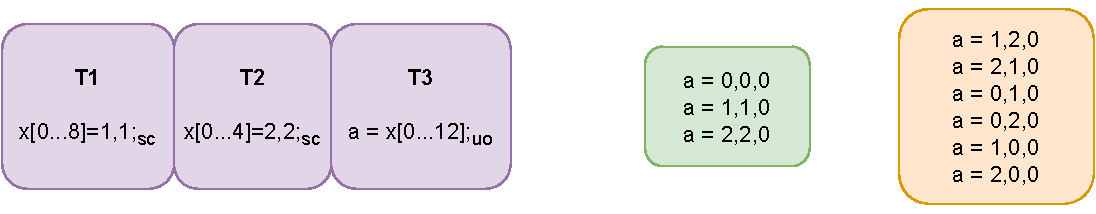
\includegraphics[scale=0.7]{6.ConclusionFutureWork/TearingExample.pdf}
            \caption{Mixed-size Tearing reads example}
            \label{crit:tearing}
        \end{figure}

        The green box represents the outcomes that we can intuitively justify.
        But the model also allows the outcomes in the orange box. 
        This is because of the read that tears, which implies that Axiom \ref{TfRe} does not constrain $\stck{_{rf}}$ to be functional with respect to the read and the writes to the same 8-byte memory. 
        Whether this is left to the hardware or program transformations is uncertain.
        If so, how could one justify any of the outcomes in the orange box is yet to be understood by us. 

        The main concern is that if both the writes are tear-free as well as sequentially consistent, how is it that the read can read them as if they are teared?
        Does this mean that the tearing factor of SC events depends on the existence of reads that tear or do not tear? 
        If this is so, it would be non-trivial to reason about programs locally.
       
        Consider the same last program above but with the read also of type $sc$. 
        Yet the above two behaviors having those read values are allowed.,
        Even Axiom \ref{SeqCsAt} does not restrict such an observable behavior.

        We believe this to be a problem with the tear-free reads axiom.
        A possible direction towards resolving this is to define the notion of tear-free / tearing using read-bytes-from relation. 

    \subsection{Range of Initialize events uncertain}

        Whether the range of $init$ events is the entire shared memory buffer or is it byte-size is uncertain.
        This affects the way we can reason with our programs and their corresponding observable behaviors.

        Consider the two candidates in Figure \ref{crit:range}, each of which could represent the same program, one where the initialize event is to the whole 8-byte (right) and one where its split into two events of type $init$ writing 4 bytes each (left).
        All accesses involved here are tear-free.
        The orange box is an observable behaviors in question.
        \begin{figure}[H]
            \centering
            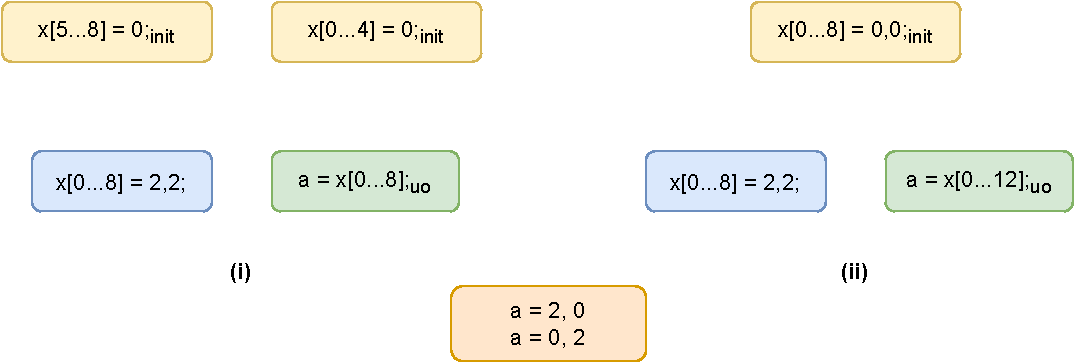
\includegraphics[scale=0.7]{6.ConclusionFutureWork/InitExample.pdf}
            \caption{Mixed-size Init events example}
            \label{crit:range}
        \end{figure}

        For the first candidate, the outcomes in question are possible.
        But for the second program, the outcomes are not possible due to Axiom \ref{TfRe}.
        Specifically, it is disallowed due to Ranges being unequal among different accesses. 
        Which one must correspond to the original program is unclear and is not specified by the semantics of the model.

    \subsection{Mixed-size events do not respect Coherence irrespective of access mode}

        Events that are unordered need not respect Coherence, unless constrained by happens-before relation.
        These accesses, mixed with sequentially consistent ones, give non-trivial behaviors.

        For instance, consider the program in Figure \ref{crit:coherence} with the orange box having the observable behavior in question.
        \begin{figure}[H]
            \centering
            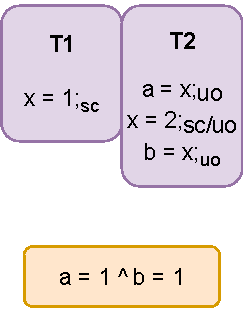
\includegraphics[scale=0.7]{6.ConclusionFutureWork/CoherenceNormal.pdf}
            \caption{Coherence violation Example.}
            \label{crit:coherence}
        \end{figure}

        The above program can have the observable behavior under question.
        But this would imply that the value of write to $x$ as $2$, though local to the subsequent read, vanishes. 
        The keen reader will note that such a behavior cannot even be explained by reordering or elimination of events as this would trivially violate the data dependency relations.
        Note also that this outcome is possible even if the write $x=2$ has an access mode of $sc$. 

        Suppose we do have standard coherence respected. 
        In this case too, sequentially consistent accesses which are mixed size give non-trivial behaviors.
        Consider another example in Figure \ref{crit:coherence_mixed} with a few mixed size accesses, where the writes are of type $sc$.
        All accesses are once again tear-free.
        \begin{figure}[H]
            \centering
            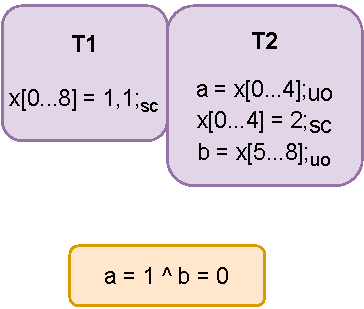
\includegraphics[scale=0.7]{6.ConclusionFutureWork/CoherenceMixed.pdf}
            \caption{Mixed-size events example where coherence is assumed to be held.}
            \label{crit:coherence_mixed}
        \end{figure}

        Here the value of read $a=x[0...4]$, despite being $1$ does not restrict the outcome of the read $b=x[5...8]$ to be $0$. 
        Again, we do not know how to justify this outcome using either safe reordering or elimination. 


\section{Future Directions in Weak Memory Consistency}

    We elicit certain problems that we consider to be foundational with respect to relaxed memory models.
    Having a concrete progress in any of these directions would in our eyes help solve problems concerning the specification of such models, compiler correctness and verification of programs with relaxed memory accesses.

    \paragraph{Specification of Mixed-Size memory models}

        Most of the work done towards addressing concerns of memory model relied on the assumption that shared memory accesses are all of the same size. 
        However, hardware does allow accesses of multiple sizes. 
        Looking at this from a relaxed memory access standpoint, the semantics of such accesses is still quite unclear. 
        Part of it is due to hardware vendors not able to decide on what kind of behaviors they want to allow for programs using such accesses, which brings the same concern for high-level programming languages. 

        This thesis is based on one such model and its impact on program transformations. 
        But this model was quite simple in that the aspect of mixed-size and their behavior for atomic accesses were semantically not defined. This may not be the case for hardware models such as ARMv8. 
        Flur et.al~\cite{Flur} give their insights on having tested and observed mixed-size behaviors in hardwares.

        One direction to go is to have a concise analysis of the validity of program transformation under mixed-size models such as ARMv8 and the new possible transformations that come along with them (like merging two accesses or splitting an access into multiple accesses.) To do this would also require formally describing the mixed size model (\cite{Flur} is for an older version of ARM model).  

    \paragraph{Transformational Specification of Memory Models}

        Using relaxed memory accesses certainly has a good impact on performance. 
        Their semantics, however, are shown to be often not so suitable for quickly assessiing their impact on program transformations done by the compiler or the hardware. 
        This thesis addressed a small part of this problem, by formalizing one such weak memory model and constructing a proof to show when a few basic program transformations are valid to perform. 

        However, over reading literature on work done in this way, it has come to our knowledge that the validity of program transformations still remains a problem. 
        As new concurrent languages come, new memory models are introduced and the validity of program transformations have to be addressed for each such model separately. 
        Instead, one way to consider going about is by describing them using program transformations. 
        Lahav et.al~\cite{Lahav2} try to do this for Total-Store-Order (TSO) and a fraction of Power memory model. They do this by describing transformationally over SC. 
        However, it is still quite limited. 
        Given the different memory models that exist today for many concurrent languages and hardware, having a formal model for the well known memory models would in our perspective be a good start. 
        It would prove useful for designing new memory models, compilers as well as understanding them from a programmer's standpoint. 
        Given the increasing use of Heterogenous hardware, it would also be useful to have an automated process of constructing a memory model parametric to the choice of program transformations we would want to do.

    \paragraph{Automation of Specification of Weak Memory Models}

        This thesis also showcased counter-examples to show that some transformations may not be safe. 
        In standard literature, such an approach is also used to explain or identify loopholes in specification of memory models. 
        Known as litmus tests, they prove useful to identify which features of weak-memory consistency does a given model have. 

        However, there is little work done in inferring specifications themselves using such litmus tests. 
        The problem is that most often it becomes difficult to concisely describe a model as a set of litmus tests.
        While a lot of work has been done in identifying key examples as litmus, the work in direction of mixed-size models has just begun. 
        Lustig et.al~\cite{Lustig} do the reverse; they construct litmus tests parametric to memory consistency models. 
        One could gain some insights from this work to do the reverse. 
        

\ \newline
\ \newline  
\hrule 
\ \newline 
\ \newline 
The advent of concurrent computation called upon a major change in how we view the executions of our programs, forcing us to move away from sequential reasoning.
With the introduction of relaxed memory consistency, this sequential reasoning became more of a hurdle.
The need for non-sequential weak memory reasoning is still not something that is viewed by many necessary, which is why we still have problems that come up with the specification of weak memory models.
This thesis is a minor contribution towards having an intuitive non-sequential reasoning about concurrent programs, in a way that also in our eyes facilitates one to quickly identify potential problems with respect to program transformations. 
A major change at the educational as well as industrial level has to come, in order to propel the transformation towards user's view of their programs not as a sequential computation machines, but as a collection of partial orders with dependencies established between program components.
We sincerely hope that this thesis helps in paving way towards that direction.
